\chapter{Metodología}\label{chapter:methodology}

En el presente capítulo se describe la metodología a seguir en esta tesis.
Primero, se describe de forma general los seis pasos que se trabajarán.
Luego, se detalla en una sección completa cada uno de estos.
Finalmente, se brindan los alcances y limitaciones de la propuesta.

Como se muestra en la \autoref{fig:pipeline}, en esta investigación se siguieron los siguientes seis pasos:
(i) preparación de simulación, 
(ii) preparación de optimización, 
(iii) optimización continua,
(iv) optimización discreta,
(v) optimización de fabricación y
(vi) preparación para fabricación.

Estos pasos se siguieron para optimizar tanto un \emph{bend} como un WDM.
Una vez preparada la simulación, la etapa de optimización (continua, discreta y de fabricación) se realizó
tres veces por cada algoritmo.
La primera ejecución usa un valor de semilla de 128, la segunda de 256 y la tercera de 512.
De esta manera se aseguró iniciar con diseños aleatorios y mantener los resultados reproducibles.

Es importante señalar que los resultados de la optimización continua se usan como punto de inicio
para la optimización discreta. Asimismo, los resultados de la optimización discreta se utilizan como
entrada para la optimización de fabricación.
Este proceso tiene como fin el mantener un buen resultado \citep{Yang2017}.


En particular, el valor de $\beta$, presente en la \autoref{eq:projection}, representa el factor discretizador de nuestros diseños.
Este valor se va incrementando en la optimización discreta y de fabricación como se muestra en la
\autoref{fig:pipeline}.

Finalmente, se realizó un posprocesamiento, análisis y conversión al
formato GDSII de los diseños mejor optimizados, esto con el fin de dejar todo preparado
para una futura etapa de fabricación de estos diseños.

En las siguientes subsecciones se explica en detalle cada una de los pasos de la metodología seguida en esta tesis.

\begin{figure}[ht]
  \centering
  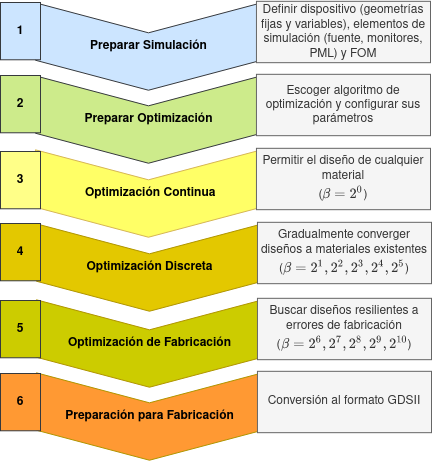
\includegraphics[scale=0.8]{image/proposal/pipeline.png}
  \caption{Metodología del trabajo de investigación}
  \label{fig:pipeline}
\end{figure}

\section{Preparación de Simulación}\label{sec:preparar-simulacion}

El \emph{bend} y WDM se parametrizaron usando la parametrización basada en píxeles descrita en la
\autoref{sec:parametrization}.
La implementación se realizó en SPINS.
La descripción detallada para los dos dispositivos de estudio se presentan en las siguientes dos subsecciones.

\subsection{\emph{Bend}}

\begin{figure}[ht]
  \centering
  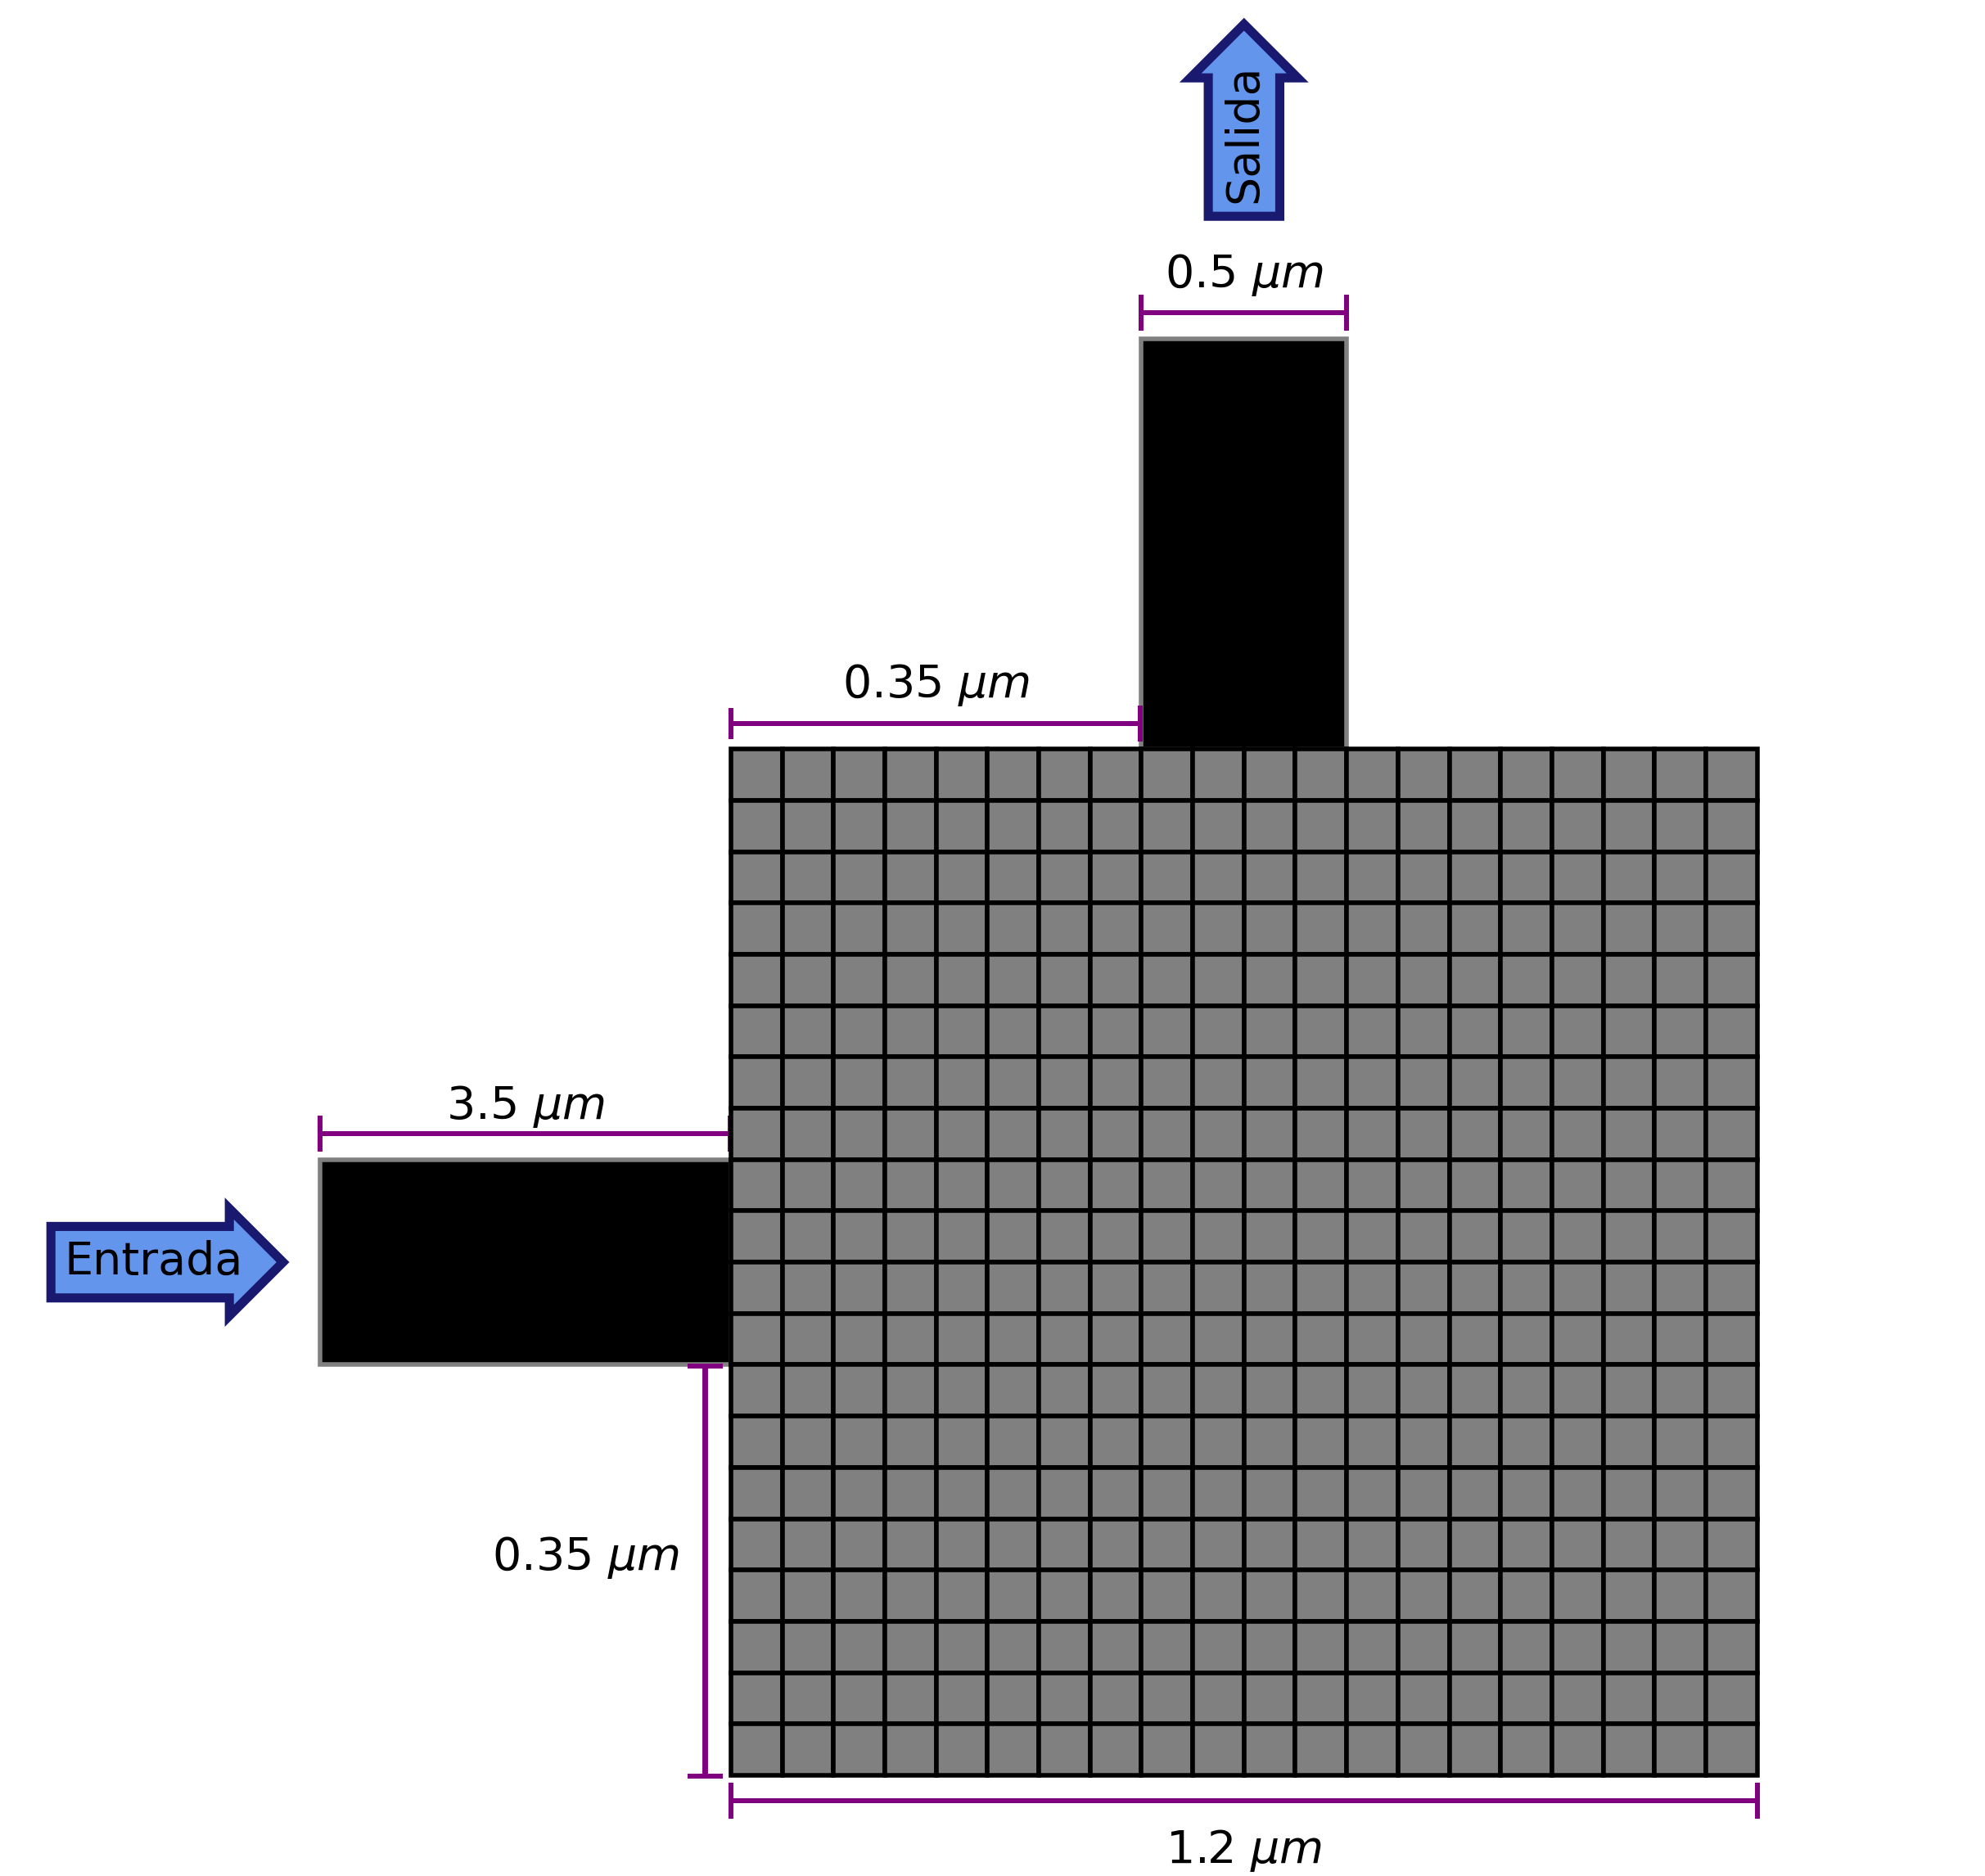
\includegraphics[width=0.6\textwidth]{image/proposal/bend.png}
  \caption{Parámetros del diseño del \emph{bend} a optimizar.}
  \label{fig:dimensiones-bend}
\end{figure}

En la \autoref{fig:dimensiones-bend} se muestra el diseño y parámetros del \emph{bend} a utilizar.
Se espera que este dispositivo trabaje a $1550 nm$.
Los rectángulo negros representan las guías de onda, estos tienen las mismas dimensiones aunque en distinta orientación.
La región gris representa la región de diseño.
La recta roja simula la fuente y la recta azul el monitor, su extensión está
simbolizada por las variables \emph{source} y \emph{monitor}, respectivamente.
Además, la profundidad de estos dos elementos es la misma, valor denotado como \emph{z\_length}.
Por otro lado, la región punteada se utiliza como referencia para definir el PML (región verde),
del cual dista un valor definido como \emph{pml\_dist}. 
La profundidad de toda la geometría es especificada por la variable \emph{depth}.

Cabe destacar que los parámetros fueron escogidos inspirados por el trabajo de \cite{Su2020}.
De este modo, la región de diseño se dividió en rectángulos de $16nm \times 16 nm$, obteniendo así una
matriz de $125 \times 125$.
Notemos que con esta configuración, en la \autoref{eq:distance} tenemos $psize_x = psize_y = 16 nm$.
El valor de los demás parámetros del diseño se presenta en la \autoref{tab:bend-values}.

\begin{table}[ht]
    \centering
    \begin{tabular}{|c|c|}
    \hline 
    Parámetro &  Valor (nm) \\
    \hline 
    wg\_height & 400 \\
    pml & 300 \\
    pml\_dist & 200 \\
    $d_1$ & 400 \\
    $d_2$ & 400 \\
    L\_width & 2000 \\
    L\_height & 2000 \\
    source & 2500 \\
    monitor & 2500 \\
    z\_length & 1000 \\
    depth & 220 \\
    \hline 
    \end{tabular}
    \caption{Parámetros usados en el diseño del \emph{bend} a optimizar.}
    \label{tab:bend-values}
\end{table}

\subsection{WDM}

\begin{figure}[ht]
  \centering
  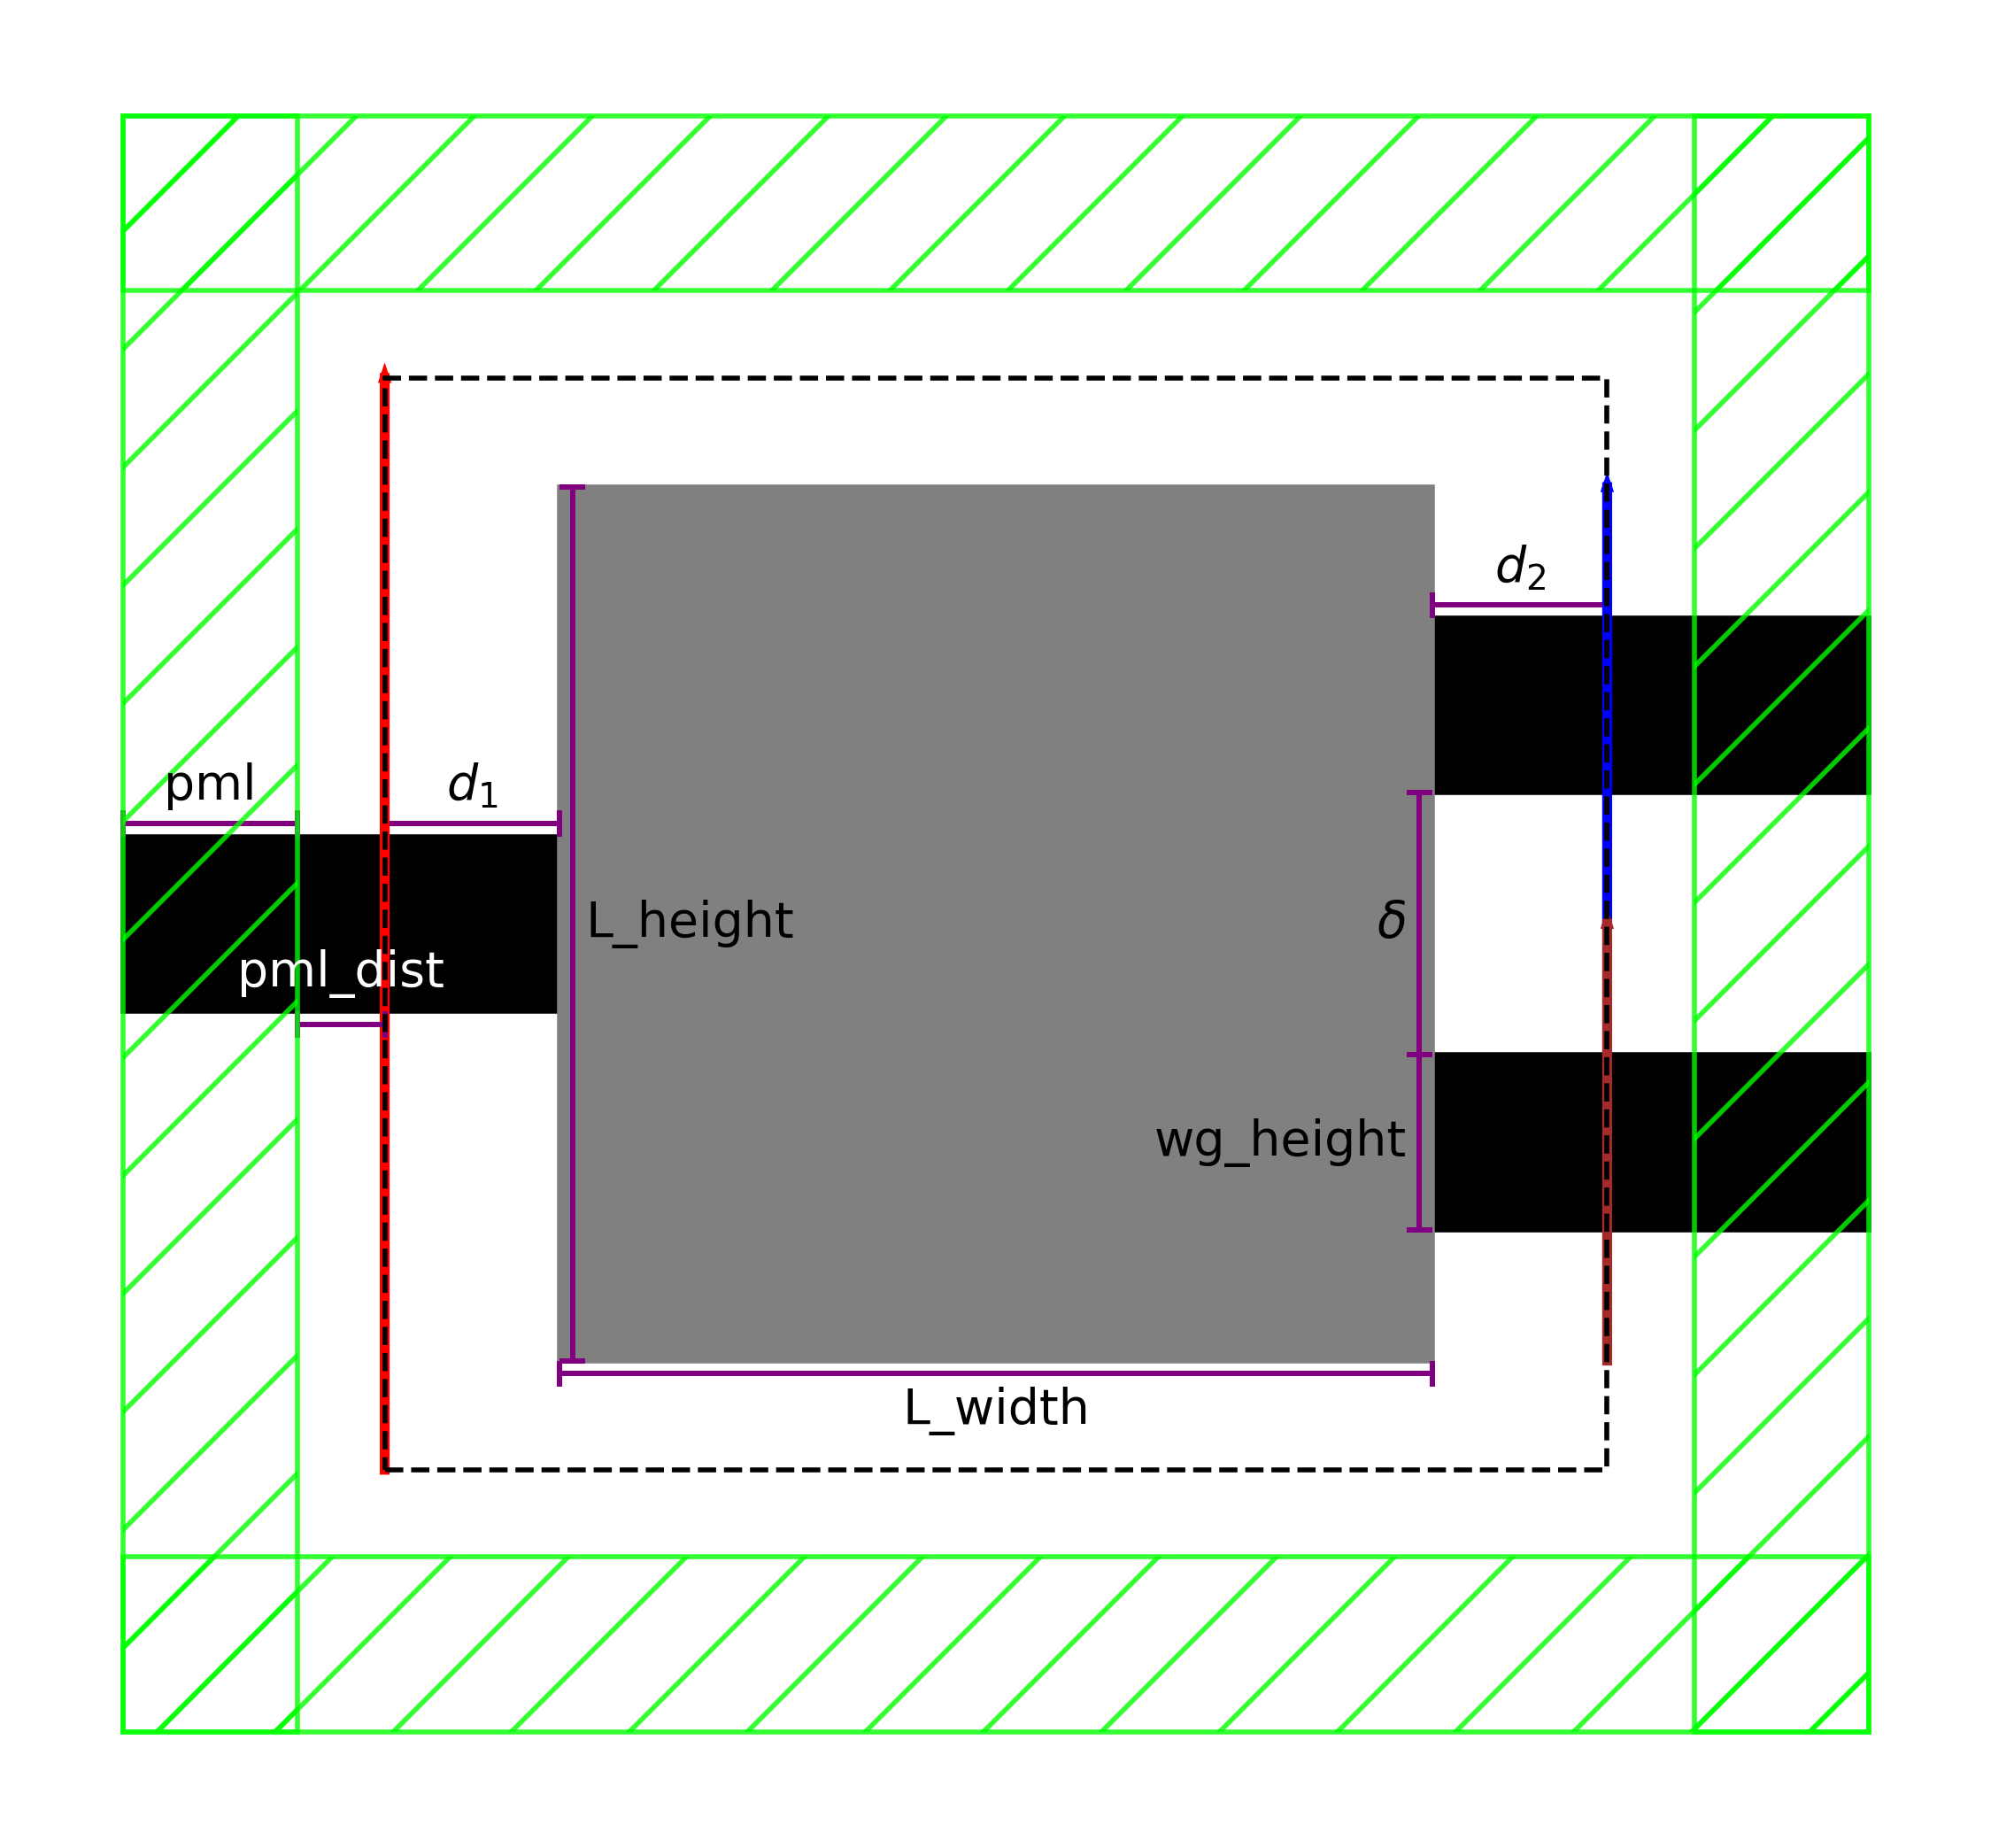
\includegraphics[width=0.6\textwidth]{image/proposal/wdm.png}
  \caption{Parámetros del diseño del WDM a optimizar.}
  \label{fig:dimensiones-demultiplexer}
\end{figure}

En la \autoref{fig:dimensiones-demultiplexer} se muestra el diseño y parámetros del WDM a utilizar.
Se espera que este dispositivo trabaje a $1300 nm$ en el brazo superior y a $1550 nm$ en el brazo inferior.
Los rectángulo negros representan las guías de onda, estos tienen las mismas dimensiones.
La región gris representa la región de diseño.
La recta roja simula la fuente y su extensión se simboliza por la variable \emph{source}.
Las rectas azul y marrón describen los monitores cuya extensión está definida por las variables \emph{monitor}.
Además, la profundidad de la fuente y monitores es la misma, denotado como \emph{z\_length}.
Por otro lado, la región punteada se utiliza como referencia para definir el PML (región verde),
del cual dista un valor definido como \emph{pml\_dist}.
La profundidad de toda la geometría es especificada por la variable \emph{depth}.

En este caso, los parámetros fueron escogidos inspirados por el trabajo de \cite{Christiansen2021}.
Del mismo modo como se realizó para el \emph{bend}, 
la región de diseño se dividió en rectángulos de $16nm \times 16 nm$, obteniendo así una
matriz de $125 \times 125$.
El valor de los demás parámetros se presenta en la \autoref{tab:wdm-values}.

\begin{table}[ht]
    \centering
    \begin{tabular}{|c|c|}
    \hline 
    Parámetro &  Valor (nm) \\
    \hline 
    wg\_height & 400 \\
    pml & 300 \\
    pml\_dist & 200 \\
    $d_1$ & 400 \\
    $d_2$ & 400 \\
    L\_width & 2000 \\
    L\_height & 2000 \\
    $\delta$ & 600 \\
    source & 2500 \\
    monitor & 1000 \\
    z\_length & 1000 \\
    depth & 220 \\
    \hline 
    \end{tabular}
    \caption{Parámetros usados en el diseño del WDM a optimizar.}
    \label{tab:wdm-values}
\end{table}


\section{Preparación de Optimización}

Con lo descrito en la anterior sección ya podemos evaluar distintos diseños.
Ahora, utilizando como función objetivo la \autoref{eq:fom-bend} para el \emph{bend} y 
la \autoref{eq:fom-splitter} para el WDM,
estamos ante un problema de optimización.
Para resolverlo, la propuesta inicial era utilizar estos cinco algoritmos:
(i) GA, (ii) PSO, (iii) CMA-ES, (iv) L-BFGS-B, (v) MMA.

La elección de estos fue por diversos motivos.
GA y PSO se escogieron por ser populares en el área \citep{Elsawy2020, Molesky2018, Prosopio-Galarza2019}.
CMA-ES por haber tenido un buen desempeño en \cite{Gregory2015} y las buenas referencias brindadas en
\cite{Campbell2019}.
L-BFGS-B por haber obtenido buenos resultados en trabajos como \cite{Su2020} y \cite{Zhang2021}.
MMA por haber sido recomendado como un buen candidato para la optimización topológica \citep{Lazarov2016}.

Por trabajos como los de \cite{Su2020}, \cite{Christiansen2021} y \cite{Lazarov2016} ya nos podíamos anticipar que al usar
L-BFGS-B o MMA se obtendrían buenos resultados en parte gracias a usar la gradiente para guiar la búsqueda.
Sin embargo, por la cantidad de variables utilizadas ($125 \times 125$) no podíamos asegurar lo mismo
con GA, PSO y CMA.

Debido a ello, primero se realizó un experimento preliminar para evaluar el desempeño de estos
algoritmos al realizar como máximo 1200 evaluaciones en la optimización del \emph{bend} propuesto, 
estos resultados son presentados en la \autoref{fig:gradient-free-comparison}.
Como podemos observar, especialmente del CMA-ES, hay una ligera tendencia de mejora.
Por otro lado, por los resultados mostrados en \cite{Christiansen2021matlab} uno esperaría que algoritmos como GA lograran 
obtener resultados similares a los obtenidos por algún algoritmo basado en la gradiente (e.g., L-BFGS-B y MMA); 
sin embargo, esto podría necesitar evaluar el FOM un número muy elevado de veces (entre $10^4$ y $10^5$).

\begin{figure}[ht]
  \centering
  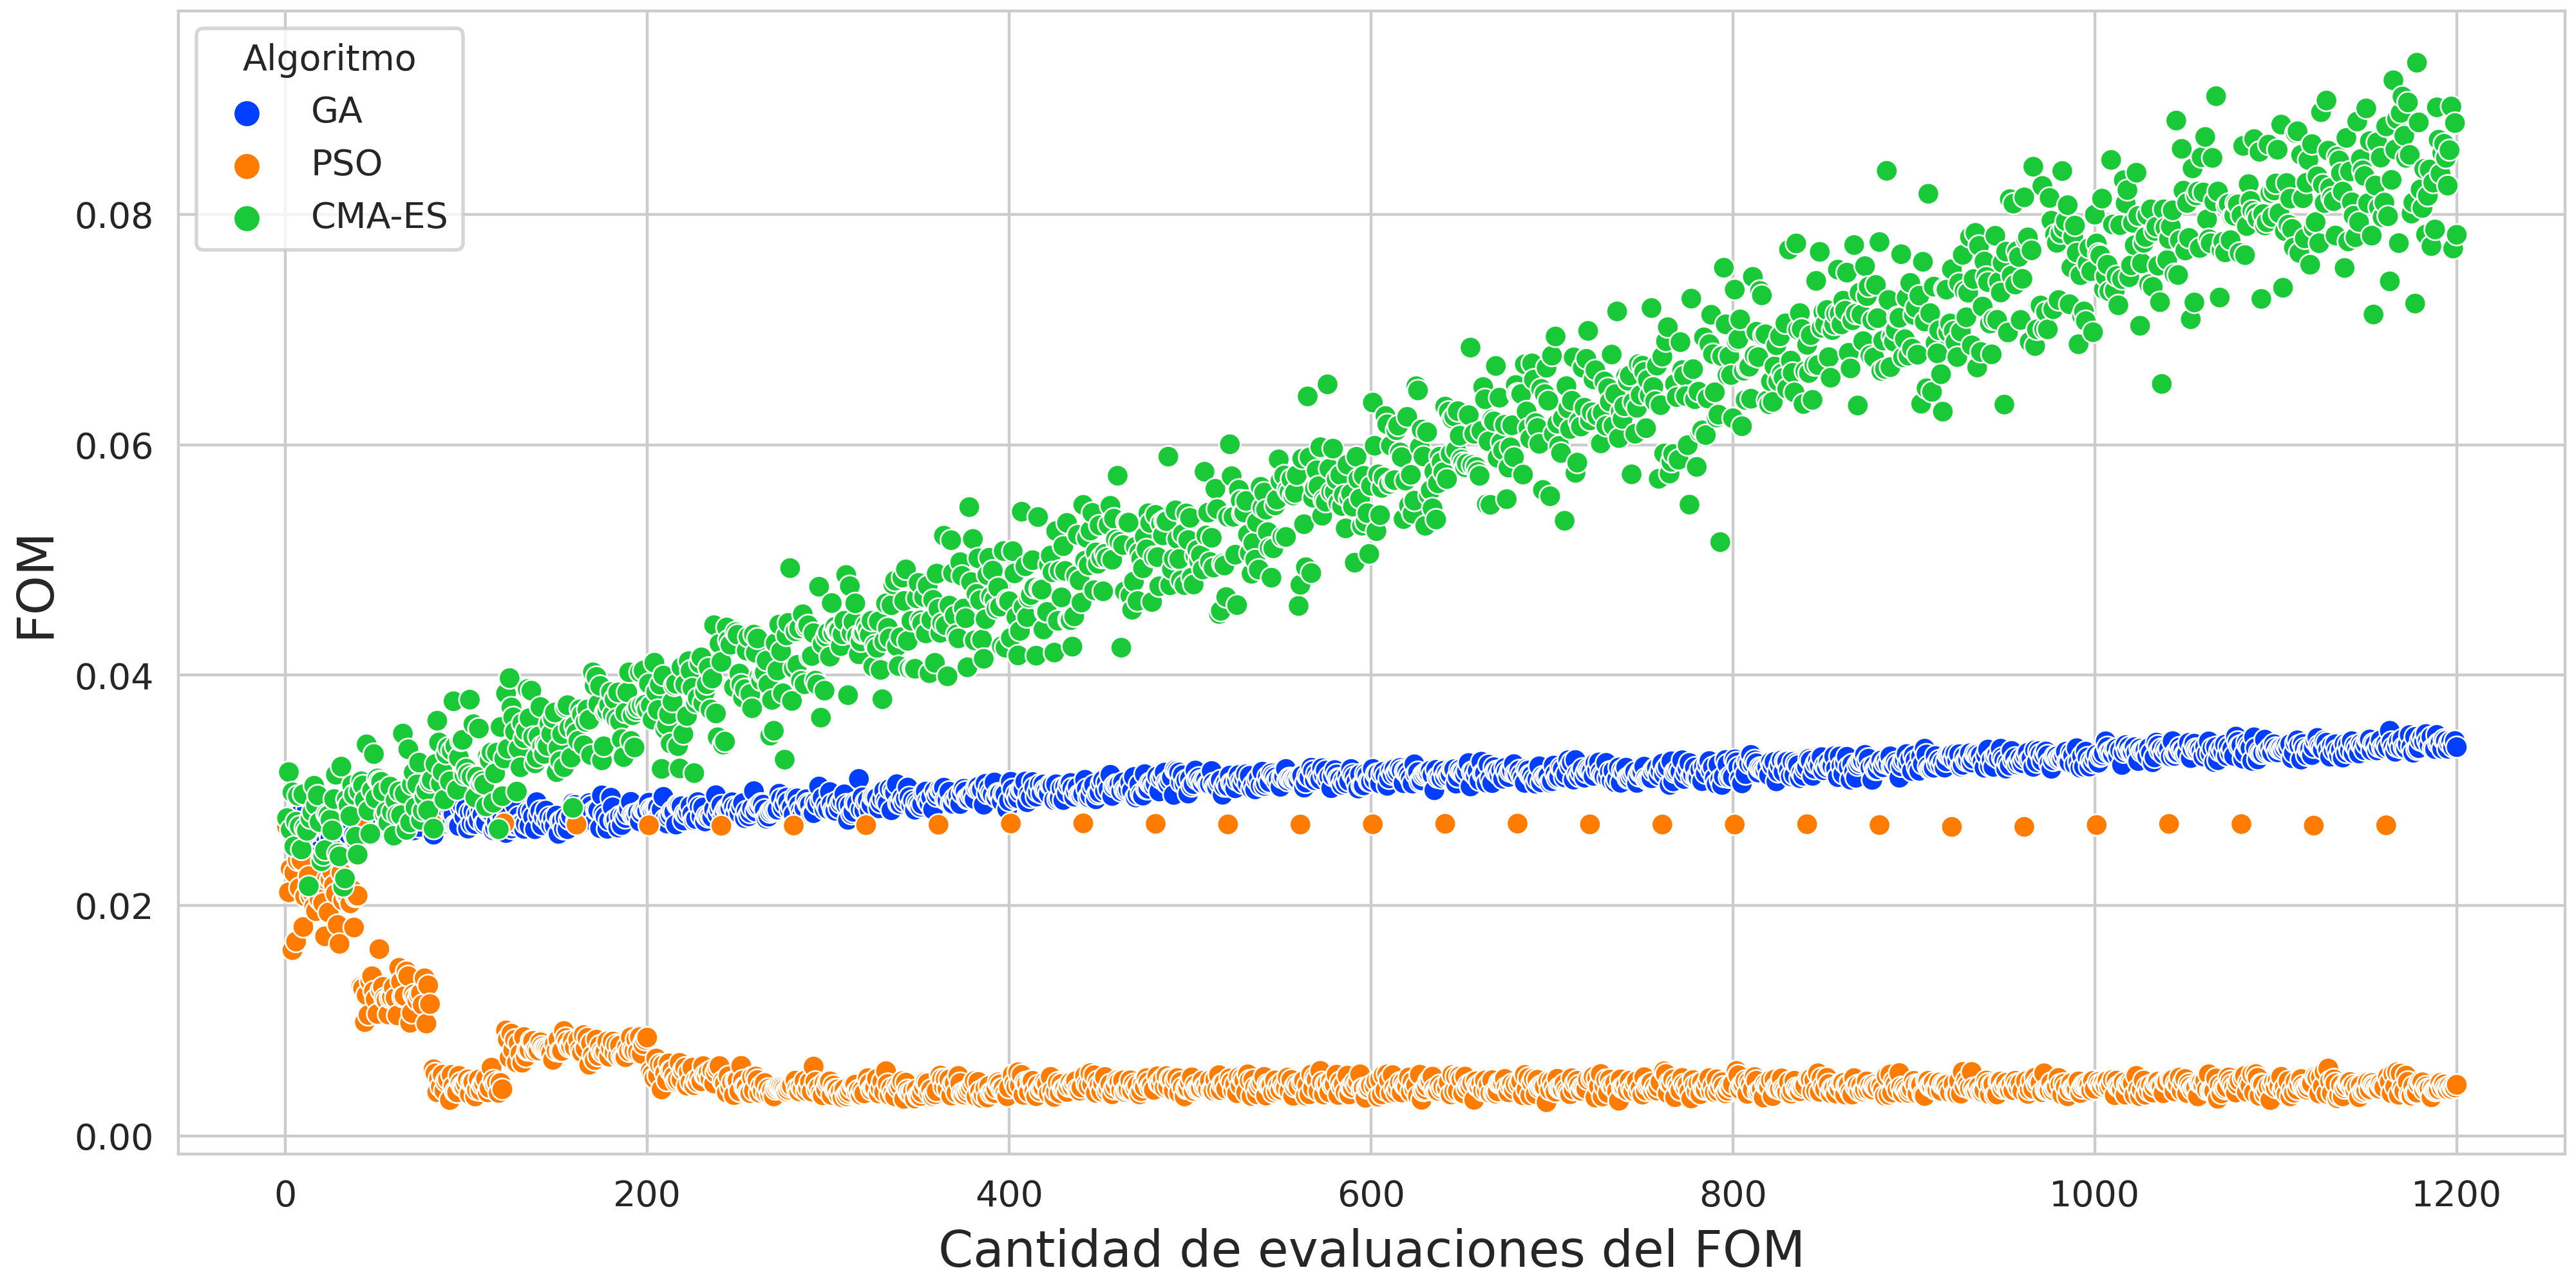
\includegraphics[width=1.0\textwidth]{image/proposal/bend-opt-cont.png}
  \caption{Comparación del desempeño de GA, PSO y CMA-ES para optimizar el \emph{bend} propuesto.}
  \label{fig:gradient-free-comparison}
\end{figure}

\begin{table}[ht]
    \centering
    \begin{tabular}{|c|c|c|}
    \hline 
    Algoritmo & Parámetro &  Valor (nm) \\
    \hline
    MMA & $m^{+}$ & 0\\
    L-BFGS-B & $\overline{m}$ & 10 \\
    L-BFGS-B & pgtol & 0 \\
    G-GA & population\_size & 40 \\
    G-GA & n\_selected\_parents & 10 \\
    G-GA & GA\_range & 0.1 \\
    G-GA & prob\_mutation & 0.1 \\
    G-PSO & population\_size & 40 \\
    G-PSO & PSO\_range & 0.1 \\
    G-PSO & $\omega$ & 0.5 \\
    G-PSO & $c_1$ & 0.5 \\
    G-PSO & $c_2$ & 0.5 \\
    G-CMA-ES & population\_size & 40 \\
    G-CMA-ES & $\sigma$ & 0.3 \\
    G-PSO & k\_gd & 10 \\
    G-PSO & gamma & 0.1\\
    G-GA & k\_gd & 10 \\
    G-GA & gamma & 0.1\\
    \hline 
    \end{tabular}
    \caption{Parámetros usados por los algoritmos de optimización.}
    \label{tab:alg-parameters}
\end{table}

De este modo, en esta tesis se optó por comparar solamente algoritmos de primer orden, es decir, que utilicen
el cómputo de la gradiente en sus rutinas. Así, se seguirá evaluando los algoritmos GA, PSO y CMA-ES pero
ahora en sus versiones que usan la gradiente.
Para poder comparar el desempeño de estos se configuró la máxima cantidad de veces que podían
evaluar la función objetivo. 
Los parámetros específicos con los que se ejecutaron cada algoritmo se detallan en la
\autoref{tab:alg-parameters} siguiendo la nomenclatura presentada en la \autoref{sec:alg-opt}.
La elección de estos parámetros es producto de la revisión de la literatura y de experimentación
propia de prueba y error.

Es resumen, usando simulaciones en 3D FDFD con SPINS-B, evaluamos estos cinco algoritmos:

\begin{enumerate}
  \item \textbf{G-PSO}
  
  Los experimentos con este algoritmo se desarrollaron con una implementación propia siguiendo lo descrito
    en \autoref{sec:g-pso}.

  \item \textbf{G-GA}


  Los experimentos con este algoritmo se desarrollaron con una implementación propia siguiendo lo descrito
    en \autoref{sec:g-ga}.

  \item \textbf{G-CMA-ES}

  Los experimentos con este algoritmo se desarrollaron usando el paquete de Python pycma
  \citep{hansen2019pycma}.

  \item \textbf{MMA} (\autoref{sec:mma})

  No se realizaron variantes en este algoritmo.
  Los experimentos se desarrollaron usando el paquete de Python NLOpt \citep{nlopt}.

  \item \textbf{L-BFGS-B} (\autoref{sec:lbfgsb})

  No se realizaron variantes en este algoritmo.
  Los experimentos se desarrollaron usando el paquete de Python SciPy \citep{2020SciPy-NMeth}.

\end{enumerate}

A continuación, se detalla la estrategia de optimización seguida en este trabajo.
Esta propuesta esta inspirada (principalmente) en el trabajo de \cite{Su2020} y \cite{Christiansen2021}.
En cada una de estas etapas se limitó la cantidad de veces que se podía evaluar $f_{obj}$ para su
posterior comparación. Además, para G-GA y G-PSO se agregó una condición para terminar el algoritmo
en caso de no encontrar mejoras mayores a $10^{-9}$ en las últimas $5$ iteraciones, 
para el L-BFGS-B se usó valores por defecto de la implementación encontrada en Scipy y 
para $MMA$ se estableció como criterio de convergencia el lograr
una tolerancia relativa de $10^{-9}$.

\section{Optimización Continua}

En esta etapa se configuró la máxima cantidad de evaluaciones a 2000.
Luego, se ejecutaron los cinco algoritmos para optimizar el \emph{bend} y WDM.
Cada algoritmo se ejecutó 3 veces, la primera con un valor de semilla de 128, la segunda de 256 y
la tercera de 512.
La idea de esta etapa es optimizar los diseños sin imponer ninguna restricción.
Es decir, directamente usamos la parametrización $\boldsymbol{P}$ para evaluar la permitividad 
$\varepsilon$ (\autoref{eq:permitivity}),
lo cual lo podemos representar como $(\boldsymbol{P} \mathrel{\leadsto} \varepsilon)$.

\section{Optimización Discreta}

Los objetivos de esta etapa son dos: (i) obtener diseños con un mínimo radio de curvatura $r_f$ e
(ii) ir eliminando las regiones grises.
Para el primer objetivo se aplicó la \autoref{eq:densityfilter} a la parametrización 
$\boldsymbol{P}$ usando un radio de curvatura $r_f = 80 nm$.
Como $80nm$ es igual a 5 veces el tamaño de los píxeles configurados en la \autoref{sec:preparar-simulacion},
solamente fue necesario explorar una submatriz de $11 \times 11$ alrededor de cada elemento para el cálculo de
esta ecuación.
Para el segundo objetivo se aplicó la \autoref{eq:projection} al resultado conseguido por el anterior filtro.
Este proceso lo podemos representar como 
$(\boldsymbol{P} \mathrel{\leadsto} \widetilde{\boldsymbol{P}} \mathrel{\leadsto}
\widetilde{\widetilde{\boldsymbol{P}}} \mathrel{\leadsto} \varepsilon)$.

Para la optimización se utilizó los resultados de la optimización continua como punto inicial.
Para ello se realizó una primera optimización configurando la máxima cantidad de evaluaciones 
en 800 y aplicando a cada diseño los filtros descritos anteriormente con $\beta = 2^1$ y $\eta = 0.5$
para la \autoref{eq:projection}.
El resultado de esta optimización se usa como punto inicial para repetir este proceso, pero ahora con $\beta
= 2^2$. Finalmente, se repite una vez más el procedimiento con $\beta = 2^3$.

\section{Optimización de Fabricación}

Por último, se busca imponer a los diseños restricciones de fabricación y robustez a posibles errores
de fabricación. 

Tomando como referencia el trabajo de \cite{Hammond20} para asegurar un buen desempeño pese a los errores de
fabricación, por cada parametrización $\boldsymbol{P}$ se calculó:

\begin{itemize}
  \item $\widetilde{\widetilde{\boldsymbol{P}}}_{d}$ que representa el diseño como si el dispositivo se hubiera dilatado.
  \item $\widetilde{\widetilde{\boldsymbol{P}}}_{i}$ que representa el diseño nomimal.
  \item $\widetilde{\widetilde{\boldsymbol{P}}}_{e}$  que representa el diseño como si el dispositivo
    hubiera erosionado.
\end{itemize}

Estos tres elementos se calcularon siguiendo los mismos filtros descritos en la anterior sección
$(\boldsymbol{P} \mathrel{\leadsto} \widetilde{\boldsymbol{P}} \mathrel{\leadsto}
\widetilde{\widetilde{\boldsymbol{P}}} \mathrel{\leadsto} \varepsilon)$.
Pero, para el diseño dilatado se usó $\eta_d = 0.45$, para el diseño nominal $\eta_i = 0.5$ y
para el diseño expandido $\eta_e = 0.55$.

Luego, se definió una nueva función objetivo mediante la siguiente ecuación:

\begin{equation}
  \begin{split}
    F_{obj} = max(min(
    f_{obj}(\widetilde{\widetilde{\boldsymbol{P}}}_{d}),
    f_{obj}(\widetilde{\widetilde{\boldsymbol{P}}}_{i}),
    f_{obj}(\widetilde{\widetilde{\boldsymbol{P}}}_{e})
    )
  \end{split}
  \label{eq:final-fom}
\end{equation}

Así, considerando el peor escenario ante dos posibles errores de fabricación (expansión o contracción),
se busca el diseño más robusto posible.
Para optimizar esta nueva función objetivo se realizó el mismo proceso de la optimización discreta, pero ahora
con valores $\beta = 2^4, 2^5, 2^6$ y limitando a 400 evaluaciones de $F_{obj}$ por cada $\beta$. 
De esta manera, en paralelo, seguimos con el proceso de discretizar
nuestros resultados.

\section{Preparación para Fabricación}

Finalmente, se seleccionó el diseño más optimo obtenido para un \emph{bend} y WDM.
Luego, se realizó un análisis del funcionamiento de estos dispositivos a distintas longitudes de onda
y se evaluó su desempeño al eliminar regiones aisladas.
Para la eliminación de regiones aisladas se realizó una búsqueda por profundidad
desde la intersección entre la guía de entrada y la región de diseño.
Para ello recorrimos la matriz $\widetilde{\widetilde{\boldsymbol{P}}}$ como un grafo implícito moviéndonos a una celda
vecina si esta poseía un valor mayor a 0.5.

Posteriormente, usando la permitividad asociada a sus parametrizationes se obtuvo la geometría del dispositivo.
Esta geometría se aproximó mediante polígonos usando el paquete \emph{mathplotlib} de Python.
Luego, se utilizaron estos polígonos con rutinas de SPINS-B
para representar el diseño en formato GDSII.
De esta manera los mejores diseños optmizados quedaron preparados para una 
futura etapa de fabricación.

\section{Alcances y Limitaciones}

El presente trabajo solo se realizó mediante simulaciones computacionales, no se llegó a la parte de
fabricación por temas de tiempo y presupuesto. Sin embargo, los mejores diseños optimizados se
encuentran listos para poder ser fabricados.

En este capítulo hemos explicado los seis pasos seguidos en esta tesis.
Primero, comenzamos describiendo la configuración de nuestros dispositivos a optimizar.
Segundo, se detalló los cinco algoritmos a utilizar, sus parámetros y justificación de elección.
Luego, se desarrolló la estrategia de optimización a seguir: optimización continua, discreta y de fabricación.
Finalmente, se describió la etapa final realizada con los mejores diseños obtenidos.
